\documentclass[12pt]{article}

\title{\vspace{-3em}PHYS 167b HW 3}
\author{Michael Cardiff}
\date{\today}

%% science symbols
\usepackage{amsmath}
\usepackage{amssymb}
\usepackage{amsthm}
\usepackage{bm}
\usepackage{cancel}
\usepackage{physics}
\usepackage{siunitx}
\usepackage{slashed}

%% general pretty stuff
\usepackage{caption}
\usepackage{float}
\usepackage{graphicx}
\usepackage{url}
\usepackage{enumitem}
\usepackage{hyperref}
\usepackage{tikz}
\usepackage{tikz-feynhand}

% setup options
\captionsetup{labelfont=bf}
\graphicspath{ {./figs/} }

% macros
\renewcommand{\L}{\mathcal{L}}
\renewcommand{\H}{\mathcal{H}}
\renewcommand{\l}{\ell}
\newcommand{\M}{\mathcal{M}}
\newcommand{\mcV}{\mathcal{V}}
\newcommand{\D}{\partial}
\newcommand{\veps}{\varepsilon}
\newcommand{\circled}[1]{\tikz[baseline=(char.base)]{
    \node[shape=circle,draw,inner sep=2pt](char){#1};}}

% mdframed environments
\usepackage[framemethod=TikZ]{mdframed}
\mdfsetup{skipabove=\topskip,skipbelow=\topskip}
\mdfdefinestyle{defstyle}{%
  linewidth=1pt,
  frametitlerule=true,
  frametitlebackgroundcolor=gray!40,
  backgroundcolor=gray!20,
  innertopmargin=\topskip
}

\mdtheorem[style=defstyle]{definition}{Definition}
\mdtheorem[style=defstyle]{theorem}{Theorem}
\mdtheorem[style=defstyle]{problem}{Problem}

\newenvironment{thebook}
{\begin{mdframed}[style=defstyle,frametitle={From the Book}]}{\end{mdframed}}

\begin{document}
\maketitle
\section{Thomson, Problem 4.1}
\begin{problem}
  Show that
  \begin{align*}
    \comm{\vu{p}^2}{\vu{r}\times\vu{p}}=0
  \end{align*}
  and hence the Hamiltonian of the free-particle Schrodinger equation commutes with the angular momentum operator.
\end{problem}
We can write out these operators as:
\begin{align*}
  \vu{p}^2&=p_xp_x+p_yp_y+p_zp_z\\
  (\vu{r}\times\vu{p})_k&=\veps_{ijk}r_ir_j\\
  (\vu{r}\times\vu{p})_1&=yp_z-zp_y\\
  (\vu{r}\times\vu{p})_2&=zp_x-xp_z\\
  (\vu{r}\times\vu{p})_3&=xp_y-yp_x
\end{align*}
We also need to use the cannonical commutation relation:
\begin{align*}
  \comm{r_j}{p_k}=i\delta_{jk}
\end{align*}
And the rule for product commutators:
\begin{align*}
  \comm{A}{BC}=\comm{A}{B}C+B\comm{A}{C}
\end{align*}
Which when we set $A=r_j$ and $B=C=p_k$:
\begin{align*}
  \comm{r_j}{p_k^2}&=\comm{r_j}{p_k}p_k+p_k\comm{r_j}{p_k}\\
  &=2ip_k\delta_{jk}
\end{align*}
This then makes the commutator easy to evaluate by components of $\vu{r}\times\vu{p}$:
\begin{align*}
  \comm{\vu{p}^2}{(\vu{r}\times\vu{p})_1}=
  \comm{p_x^2}{yp_z-zp_y}+\comm{p_y^2}{yp_z-zp_y}+\comm{p_z^2}{yp_z-zp_y}
\end{align*}
The $p_x^2$ trivially commutes, the others can be written:
\begin{align*}
  \comm{\vu{p}^2}{(\vu{r}\times\vu{p})_1}&=
  \comm{p_y^2}{y}p_z-z\comm{p_y^2}{p_y}
  +y\comm{p_z^2}{p_z}-\comm{p_z^2}{z}p_y\\
  &=2ip_yp_z-2ip_zp_y=0
\end{align*}
The cancellation comes from the fact that components of the angular momentum operators commute.

Similarly for 2, we get the $y$ term from $\vu{p}^2$ trivially commuting:
\begin{align*}
  \comm{\vu{p}^2}{(\vu{r}\times\vu{p})_2}&=
  \comm{p_x^2}{zp_x-xp_z}+\comm{p_z^2}{zp_x-xp_z}\\
  &=\comm{p_z^2}{z}p_x-\comm{p_x^2}{x}p_z\\
  &=2ip_zp_x-2ip_xp_z=0
\end{align*}
And for 3, the same applies, where instead we get:
\begin{align*}
  \comm{\vu{p}^2}{(\vu{r}\times\vu{p})_2}&=
  2ip_xp_y-2ip_yp_x=0
\end{align*}
Hence:
\begin{equation}
  \label{eq:p1a}
  \comm{\vu{p}^2}{\vu{r}\times\vu{p}}=\vb{0}
\end{equation}
And since the free particle Hamiltonian for the Schrodinger Equation is just $\hat{H}_{free}=\vu{p}^2/2m$, and the angular momentum is given by $\vu{L}=\vu{r}\times\vu{p}$, so we can conclude:
\begin{equation}
  \label{eq:p1b}
  \boxed{\comm{\hat{H}_{free}}{\vu{L}}=\vb{0}}
\end{equation}
\newpage
\section{Thomson, Problem 4.3}
\begin{problem}
  Verify the statement that the Einstein energy-momentum relationship is recovered if any of the four Dirac spinors of (4.48) are substituted into the Dirac equation written in terms of momentum $(\gamma^\mu p_\mu-m)u=0$.
\end{problem}
We can find the matrix form of $\gamma^\mu p_\mu$ using the Dirac-Pauli representation:
\begin{align*}
  \gamma^\mu p_\mu&=
  E\pmqty{\dmat{1,1,-1,-1}}
  -p_x\pmqty{\admat{1,1,-1,-1}}\\
  &-p_y\pmqty{\admat{-i,i,i,-i}}
  -p_z\pmqty{&&1\\&&&-1\\-1\\&1}\\
  &=\pmqty{
    E&0&-p_z&-p_x+ip_y\\
    0&E&-(p_x+ip_y)&p_z\\
    p_z&p_x-ip_y&-E&0\\
    p_x+ip_y&-p_z&0&-E
  }
\end{align*}
Adding in the identity term from $-m\bm{1}$:
\begin{align*}
  \gamma^\mu p_\mu-m=\pmqty{
    E-m&0&-p_z&-p_x+ip_y\\
    0&E-m&-(p_x+ip_y)&p_z\\
    p_z&p_x-ip_y&-(E+m)&0\\
    p_x+ip_y&-p_z&0&-(E+m)
  }=D
\end{align*}
Call this operator $D$ (for Dirac), we will then evaluate $D u_1$ and $D u_2$:
\begin{align*}
  D u_1&= D \qty(N\pmqty{1\\0\\p_z/(E+m)\\(p_x+ip_y)/(E+m)})\\
  &=N\pmqty{
    E-m+((-p_x+ip_y)(p_x+ip_y)-p_z^2)/(E+m)\\
    (-(p_x+ip_y)p_z+(p_x+ip_y)p_z)/(E+m)\\
    p_z-(E+m)p_z/(E+m)\\
    p_x+ip_y-(E+m)(p_x+ip_y)/(E+m)
  }\\
  &=N\pmqty{
    E-m+(-p_x^2-p_y^2-p_z^2)/(E+m)\\
    0\\ 0\\ 0
  }
  =\frac{N}{E+m}\pmqty{p^\mu p_\mu-m^2\\0\\0\\0}
\end{align*}
Which is only valid if the Einstein-Energy relation is recovered from the first component.

The corresponding algebra for $u_2$ is:
\begin{align*}
  D u_2&= D \qty(N\pmqty{0\\1\\(p_x-ip_y)/(E+m)\\-p_z/(E+m)})
\end{align*}
Which results in the second component getting the energy momentum relation:
\begin{align*}
  D u_2&=\frac{N}{E+m}\pmqty{0\\p^\mu p_\mu-m^2\\0\\0}
\end{align*}
Similarly, $u_3$ and $u_4$ get the relation in the third and fourth components of the spinor respectively:
\begin{align*}
  D u_3&=\frac{N}{E+m}\pmqty{0\\0\\p^\mu p_\mu-m^2\\0}\\
  D u_4&=\frac{N}{E+m}\pmqty{0\\0\\0\\p^\mu p_\mu-m^2}
\end{align*}
Hence for each of the four $u$ spinors (call them collectively $u_i$), we have shown that:
\begin{equation}
  \label{eq:p2}
  \boxed{(\gamma^\mu p_\mu-m)u_i=0\implies p^\mu p_\mu-m^2=0}
\end{equation}
\newpage
\section{Thomson, Problem 4.7}
\begin{problem}
  By operating on the Dirac equation,
  \begin{align*}
    (i\gamma^\mu\D_\mu-m)\psi=0
  \end{align*}
  With $\gamma^\nu\D_\nu$, prove that the components of $\psi$ satisfy the Klein-Gordon equation,
  \begin{align*}
    (\D^\mu\D_\mu+m^2)\psi=0
  \end{align*}
\end{problem}
Rewrite the Dirac equation:
\begin{align*}
  i\gamma^\mu\D_\mu\psi=m\psi\implies\gamma^\mu\D_\mu\psi=-im\psi
\end{align*}
Operate on the left with $\gamma^\nu\D_\nu$:
\begin{align*}
  \gamma^\nu\D_\nu\qty(i\gamma^\mu\D_\mu\psi)&=\gamma^\nu\D_\nu(m\psi)
  =m(\gamma^\nu\D_\nu\psi)=m(-im\psi)\\
  i\gamma^\nu\D_\nu\gamma^\mu\D_\mu&=-im^2\psi
\end{align*}
Since derivatives commute, we can swap the places of these two derivatives, allowing for:
\begin{align*}
  \gamma^\nu\D_\nu\gamma^\mu\D_\mu=\gamma^\nu\gamma^\mu\D_\nu\D_\mu
  =\gamma^\mu\gamma^\nu\D_\mu\D_\nu
\end{align*}
By renaming indices cleverly, we can equivalently write this as:
\begin{align*}
  \gamma^\nu\D_\nu\gamma^\mu\D_\mu=
  \frac12(\gamma^\nu\D_\nu\gamma^\mu\D_\mu+\gamma^\mu\D_\nu\gamma^\nu\D_\mu)
  =\frac12(\gamma^\nu\gamma^\mu+\gamma^\mu\gamma^\nu)\D_\mu\D_\nu
\end{align*}
This is the anticommutator for the gamma matrices, which has a closed form:
\begin{align*}
  \acomm{\gamma^\mu}{\gamma^\nu}=2g^{\mu\nu}
\end{align*}
Allowing us to write:
\begin{align*}
  \gamma^\nu\D_\nu\gamma^\mu\D_\mu=g^{\mu\nu}\D_\mu\D_\nu=\D^\mu\D_\mu
\end{align*}
Hence replacing the term in our modified Dirac equation:
\begin{align*}
  i\D^\mu\D_\mu\psi=-im^2\psi\implies \D^\mu\D_\mu\psi=-m^2\psi
\end{align*}
Therefore, we recover the Dirac equation:
\begin{equation}
  \label{eq:p3}
  \boxed{(\D^\mu\D_\mu+m^2)\psi=0}
\end{equation}
\newpage
\section{Thomson, Problem 4.10}
\begin{problem}
  Demonstrate that the two relations of Equation (4.45) are consistent by showing that:
  \begin{align*}
    (\bm{\sigma}\vdot\vb{p})^2=\vb{p}^2
  \end{align*}
\end{problem}
We can begin by expanding the term on the left hand side:
\begin{align*}
  (\bm{\sigma}\vdot\vb{p})^2&=
  (\sigma_xp_x+\sigma_yp_y+\sigma_zp_z)^2\\
  &=\sigma_x^2p_x^2+\sigma_y^2p_y^2+\sigma_z^2p_z^2\\
  &+\sigma_xp_x\sigma_yp_y+\sigma_xp_x\sigma_zp_z\\
  &+\sigma_yp_y\sigma_xp_x+\sigma_yp_y\sigma_zp_z\\
  &+\sigma_zp_z\sigma_xp_x+\sigma_zp_z\sigma_yp_y
\end{align*}
Notice that since the $p_i$ are all numbers, we can write the cross terms as anticommutators of Pauli matrices, which are all zero here, so we have:
\begin{align*}
  (\bm{\sigma}\vdot\vb{p})^2&=\sigma_x^2p_x^2+\sigma_y^2p_y^2+\sigma_z^2p_z^2
\end{align*}
Since the Pauli matrices all square to the identity, we are left with:
\begin{align*}
  (\bm{\sigma}\vdot\vb{p})^2&=p_x^2+p_y^2+p_z^2=\vb{p}^2
\end{align*}
Hence we have recovered:
\begin{equation}
  \label{eq:p4}
  \boxed{(\bm{\sigma}\vdot\vb{p})^2=\vb{p}^2}
\end{equation}
\newpage
\section{Thomson, Problem 4.12}
\begin{problem}
  Verify that the helicity operator:
  \begin{align*}
    \hat{h}=\frac{\vu{\Sigma}\vdot\vu{p}}{2p}=\frac1{2p}\pmqty{\bm{\sigma}\vdot\vu{p}&0\\0&\bm{\sigma}\vdot\vu{p}}
  \end{align*}
  Commutes with the Dirac Hamiltonian:
  \begin{align*}
    \hat{H}_D=\bm{\alpha}\vdot\vu{p}+\beta m
  \end{align*}
\end{problem}
Note that in the Dirac-Pauli basis, the $\bm{\alpha}$ and $\beta$ matrices are:
\begin{align*}
  \alpha_i=\pmqty{0&\sigma_i\\\sigma_i&0}\qquad
  \beta=\pmqty{\bm{1}&0\\0&-\bm{1}}
\end{align*}
Since the $\beta$ matrix is essentially an identity matrix, it trivially commutes with anything, so we only need to compute $\comm{\hat{h}}{\bm{\alpha}\vdot\vu{p}}$:
\begin{align*}
  \comm{\hat{h}}{\bm{\alpha}\vdot\vu{p}}\propto
  \pmqty{\bm{\sigma}\vdot\vu{p}&0\\0&\bm{\sigma}\vdot\vu{p}}
  \pmqty{0&\bm{\sigma}\vdot\vu{p}\\\bm{\sigma}\vdot\vu{p}&0}-
  \pmqty{0&\bm{\sigma}\vdot\vu{p}\\\bm{\sigma}\vdot\vu{p}&0}
  \pmqty{\bm{\sigma}\vdot\vu{p}&0\\0&\bm{\sigma}\vdot\vu{p}}
\end{align*}
The first product is given by:
\begin{align*}
  \pmqty{\bm{\sigma}\vdot\vu{p}&0\\0&\bm{\sigma}\vdot\vu{p}}
  \pmqty{0&\bm{\sigma}\vdot\vu{p}\\\bm{\sigma}\vdot\vu{p}&0}
  =\pmqty{0&(\bm{\sigma}\vdot\vu{p})^2\\(\bm{\sigma}\vdot\vu{p})^2&0}
\end{align*}
And the other:
\begin{align*}
  \pmqty{0&\bm{\sigma}\vdot\vu{p}\\\bm{\sigma}\vdot\vu{p}&0}
  \pmqty{\bm{\sigma}\vdot\vu{p}&0\\0&\bm{\sigma}\vdot\vu{p}}
  =\pmqty{0&(\bm{\sigma}\vdot\vu{p})^2\\(\bm{\sigma}\vdot\vu{p})^2&0}
\end{align*}
Hence they cancel out, and we find:
\begin{equation}
  \label{eq:p5}
  \boxed{\comm{\hat{h}}{\hat{H}_D}=0}
\end{equation}
\newpage
\section{Thomson, Problem 4.14}
\begin{problem}
  Under the combined operation of parity and charge conjugation ($\hat{C}\hat{P}$) spinors transform as:
  \begin{align*}
    \psi\to\psi^c=\hat{C}\hat{P}\psi=i\gamma^2\gamma^0\psi^*
  \end{align*}
  Show that up to an overall complex phase factor:
  \begin{align*}
    \hat{C}\hat{P}u_{\uparrow}(\theta,\phi)=v_{\downarrow}(\pi-\theta,\pi+\phi)
  \end{align*}
\end{problem}
Reminder, the form of the two spinors are:
\begin{align*}
  u_{\uparrow}(\theta,\phi)=N
  \pmqty{c\theta/2\\e^{i\phi}s\theta/2\\
    \alpha c\theta/2\\\alpha e^{i\phi} s\theta/2}
  \qquad
  v_{\downarrow}(\theta,\phi)=N
  \pmqty{\alpha c\theta/2\\\alpha e^{i\phi}s\theta/2\\
    c\theta/2\\ e^{i\phi} s\theta/2}
\end{align*}
Where:
\begin{align*}
  N=\sqrt{E+m}\quad\alpha=\frac{p}{E+m}\quad c\equiv\cos\quad s\equiv\sin
\end{align*}
We then need the form of the matrix used for the combined $CP$ transform, using the explicit forms of the $\gamma$ matrices
\begin{align*}
  i\gamma^2=\pmqty{&&&1\\&&-1&\\&-1&&\\1&&&}
  \qquad
  \gamma^0=\pmqty{1\\&1\\&&-1\\&&&-1}
\end{align*}
The combination is then:
\begin{align*}
  i\gamma^2\gamma^0=
  \pmqty{&&&1\\&&-1&\\&-1&&\\1&&&}\pmqty{1\\&1\\&&-1\\&&&-1}
  =\pmqty{&&&-1\\&&1&\\&-1&&\\1&&&}
\end{align*}
Therefore we can write $\hat{C}\hat{P}u_\uparrow$ as:
\begin{align*}
  \hat{C}\hat{P}u_\uparrow=N\pmqty{&&&-1\\&&1&\\&-1&&\\1&&&}
  \pmqty{c\theta/2\\e^{-i\phi}s\theta/2\\
    \alpha c\theta/2\\\alpha e^{-i\phi} s\theta/2}=
  N\pmqty{-\alpha e^{-i\phi}s\theta/2\\\alpha c\theta/2\\
    -e^{-i\phi}s\theta/2\\c\theta/2}
\end{align*}
We can then look at $v_\downarrow(\pi-\theta,\pi+\phi)$:
\begin{align*}
  v_\downarrow(\pi-\theta,\pi+\phi)=N
  \pmqty{\alpha c(\pi-\theta)/2\\\alpha e^{i(\phi+\pi)}s(\pi-\theta)/2\\
    c(\pi-\theta)/2\\ e^{i(\pi+\phi)} s(\pi-\theta)/2}
\end{align*}
We can simplify these using the periodic and coupled nature of $\sin$ and $\cos$:
\begin{align*}
  c(\pi-\theta)/2&=s\theta/2\\
  s(\pi-\theta)/2&=c\theta/2\\
  e^{i(\pi+\phi)}=e^{i\pi}e^{i\phi}&=-e^{i\phi}
\end{align*}
Resulting in:
\begin{align*}
  v_\downarrow(\pi-\theta,\pi+\phi)&=N
  \pmqty{\alpha s\theta/2\\-\alpha e^{i\phi}c\theta/2\\
    s\theta/2\\ -e^{i\phi} c\theta/2}\\
  &=-e^{i\phi}N\pmqty{\alpha e^{-i\phi}s\theta/2\\\alpha c\theta/2\\
    -e^{-i\phi}s\theta/2\\ c\theta/2}
\end{align*}
Notice that this is exactly what we found to be $\hat{C}\hat{P}u_\uparrow(\theta,\phi)$, with a complex phase, hence we verified:
\begin{equation}
  \label{eq:p6}
  \boxed{
    \hat{C}\hat{P}u_{\uparrow}(\theta,\phi)=v_{\downarrow}(\pi-\theta,\pi+\phi)}
\end{equation}
\newpage
\section{Thomson, Problem 5.3}
\begin{problem}
  Draw the lowest-order $t$-channel and $u$-channel Feynman diagrams for $e^+e^-\to\gamma\gamma$ and use the Feynman rules for QED to write down the corresponding matrix elements
\end{problem}
The lowest-order diagrams here are simple tree-level diagrams, given in figure \Ref{fig:diagrams}:
\begin{figure}[H]
  \centering
  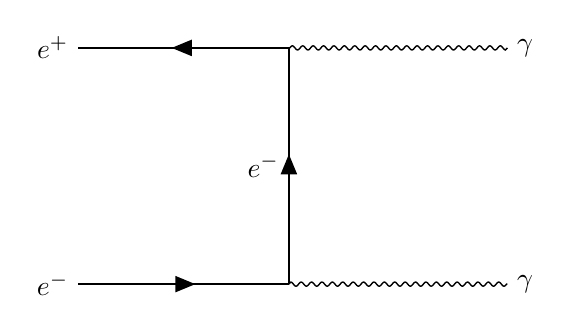
\begin{tikzpicture}[scale=2.0]
    \begin{feynhand}
      % vertices
      \vertex (p11) at (1.5,0) {$\gamma$};
      \vertex (p21) at (1.5,1.5) {$\gamma$};
      \vertex (p12) at (-1.5,0) {$e^-$};
      \vertex (p22) at (-1.5,1.5) {$e^+$};
      \vertex (a) at (0,0); \vertex (b) at (0,1.5);
      % particles
      \propag [fer] (p12) to (a);
      \propag [fer] (b) to (p22);
      \propag [bos] (b) to (p21);
      \propag [bos] (p11) to (a);
      % transfer
      \propag [fer] (a) to [edge label=\(e^-\)] (b);
    \end{feynhand}
  \end{tikzpicture}
  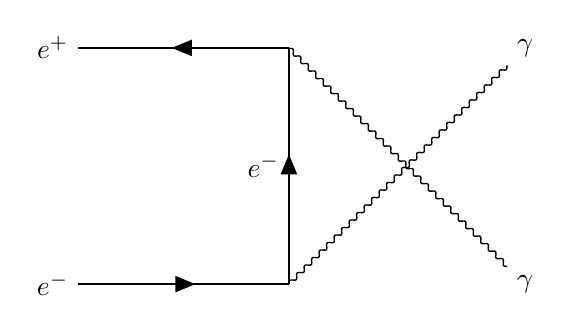
\begin{tikzpicture}[scale=2.0]
    \begin{feynhand}
      % vertices
      \vertex (p11) at (1.5,0) {$\gamma$};
      \vertex (p21) at (1.5,1.5) {$\gamma$};
      \vertex (p12) at (-1.5,0) {$e^-$};
      \vertex (p22) at (-1.5,1.5) {$e^+$};
      \vertex (a) at (0,0); \vertex (b) at (0,1.5);
      % particles
      \propag [bos] (p21) to (a);
      \propag [fer] (p12) to (a);
      \propag [bos] (b) to (p11);
      \propag [fer] (b) to (p22);
      % loop
      \propag [fer] (a) to [edge label=\(e^-\)] (b);
    \end{feynhand}
  \end{tikzpicture}
  \caption{Lowest order (Left) $t$-channel and (Right) $u$-channel Diagrams}
  \label{fig:diagrams}
\end{figure}
Let the electron momentum in both cases be $p_1$, and the positron momentum  be $p_2$, and the ``top'' $\gamma$ have momentum $p_4$ and the ``bottom'' one have $p_3$, this means that for the $t$-channel diagram, the momentum transfer $q$ is given by $q=p_1-p_3$, and for the $u$-channel diagram $q=p_1-p_4$, corresponding to the appropriate Mandelstam invariants.

The ``raw'' matrix element for the $t$-channel diagram is then given by:
\begin{align*}
  -i\M^{(t)}&=\qty[\veps^*_\mu(p_3)(-ieQ_e)\gamma^\mu u(p_1)]\\
  &\times\qty[-\frac{i(\gamma^\delta q_\delta+m_e)}{q^2-m_e}]\\
  &\times\qty[\bar{v}(p_2)(-ieQ_e)\gamma^\nu \veps^*_\nu(p_4)]
\end{align*}
This can be simplified by recalling that $Q_e$ is just a number, more importantly that it squares to $1$, and we only have a single overall minus sign from the propagator:
\begin{equation}
  \label{eq:p7a}
  \boxed{
    \begin{aligned}
      i\M^{(t)}&=-ie^2\qty[\veps^*_\mu(p_3)\gamma^\mu u(p_1)]
      \qty[\frac{(\gamma^\delta(p_1-p_3)_\delta+m_e)}{(p_1-p_3)^2-m_e}]
      \qty[\bar{v}(p_2)\gamma^\nu \veps^*_\nu(p_4)]
    \end{aligned}
  }
\end{equation}
The ``raw'' diagram for the $u$-channel diagram just has its momentum rearranged:
\begin{align*}
  -i\M^{(u)}&=\qty[\veps^*_\mu(p_4)(-ieQ_e)\gamma^\mu u(p_1)]\\
  &\times\qty[-\frac{i(\gamma^\delta q_\delta+m_e)}{q^2-m_e}]\\
  &\times\qty[\bar{v}(p_2)(-ieQ_e)\gamma^\nu \veps^*_\nu(p_3)]
\end{align*}
Hence, we can similarly simplify it:
\begin{equation}
  \label{eq:p7b}
  \boxed{
    \begin{aligned}
      i\M^{(u)}&=-ie^2\qty[\veps^*_\mu(p_4)\gamma^\mu u(p_1)]
      \qty[\frac{(\gamma^\delta(p_1-p_4)_\delta+m_e)}{(p_1-p_4)^2-m_e}]
      \qty[\bar{v}(p_2)\gamma^\nu \veps^*_\nu(p_3)]
    \end{aligned}
  }
\end{equation}
\newpage
\section{Thomson, Problem 4.9}
\begin{problem}
  Starting from:
  \begin{align*}
    (\gamma^\mu p_\mu-m)u=0
  \end{align*}
  Show that the corresponding equation for the adjoint spinor is
  \begin{align*}
    \bar{u}(\gamma^\mu p_\mu-m)=0
  \end{align*}
  Hence, without using the explicit form for the $u$ spinors, show that the normalization condition $u^\dag u=2E$ leads to:
  \begin{align*}
    \bar{u}u=2m
  \end{align*}
  and that
  \begin{align*}
    \bar{u}\gamma^\mu u=2p^\mu
  \end{align*}
\end{problem}
In momentum space, the Dirac equation is given by:
\begin{align*}
  (\gamma^\mu p_\mu-m)u=0
\end{align*}
We can take the Hermitian conjugate of both sides, noting that $m$ and $p_\mu$ are both just numbers:
\begin{align*}
  u^\dag((\gamma^\mu)^\dag p_\mu-m)=0
\end{align*}
We can use the property of the gamma matrices that:
\begin{align*}
  (\gamma^\mu)^\dag=\gamma^0\gamma^\mu\gamma^0
\end{align*}
In order to get rid of the Hermitian conjugate:
\begin{align*}
  u^\dag(\gamma^0\gamma^\mu\gamma^0 p_\mu-m)=0
\end{align*}
If we insert an identity $\bm{1}=\gamma^0\gamma^0$, we can factor out a $\gamma^0$ to turn the $u^\dag$ into a $\bar{u}$:
\begin{align*}
  \bar{u}(\gamma^\mu\gamma^0 p_\mu-m\gamma^0)
  =\bar{u}(\gamma^\mu p_\mu-m)\gamma^0=0
\end{align*}
We can then multiply by $\gamma^0$ on the right on both sides to get rid of the extra $\gamma^0$, hence we find the Dirac equation for the adjoint spinor $\bar{u}$:
\begin{equation}
  \label{eq:p8a}
  \boxed{\bar{u}(\gamma^\mu p_\mu-m)=0}
\end{equation}
For the next part, consider both the Dirac equation for the regular and adjoint spinor:
\begin{align*}
  \bar{u}(\gamma^\mu p_\mu-m)&=0\\
  (\gamma^\mu p_\mu-m)u&=0
\end{align*}
In order to use the normalization, we will need a $\gamma^0$ involved, and these equations both lack one of the spinors we need, so multiply the adjoint equation by $\gamma^0u$ on the right, and the non-adjoint equation by $\bar{u}\gamma^0$ on the left:
\begin{align*}
  \bar{u}(\gamma^\mu p_\mu-m)\gamma^0u&=0\\
  \bar{u}\gamma^\mu\gamma^0p_\mu u-m\bar{u}\gamma^0u&=0\\
  \bar{u}\gamma^0(\gamma^\mu p_\mu-m)u&=0\\
  \bar{u}\gamma^0\gamma^\mu p_\mu u-m\bar{u}\gamma^0u&=0
\end{align*}
Add the equations together:
\begin{align*}
  \bar{u}(\gamma^\mu\gamma^0+\gamma^0\gamma^\mu)p_\mu u-2m\bar{u}\gamma^0u=0
\end{align*}
Sub in the anticommutator $\acomm{\gamma^\mu}{\gamma^\nu}=2g^{\mu\nu}$:
\begin{align*}
  2\bar{u}g^{\mu0}p_\mu u-2m\bar{u}\gamma^0u=
  2\bar{u}p^0 u-2m\bar{u}\gamma^0u=0
\end{align*}
Notice that since $\bar{u}=u^\dag\gamma^0$, we recover the normalization when considering the right hand term:
\begin{align*}
  E\bar{u}u=mu^\dag u=2mE
\end{align*}
Hence with one last bit of algebra we get the desired result:
\begin{equation}
  \label{eq:p8b}
  \boxed{\bar{u}u=2m}
\end{equation}
If we had instead multiplied by $\gamma^\nu$ instead of just $\gamma^0$, we would have recovered:
\begin{align*}
  p^\nu\bar{u}u=m\bar{u}\gamma^\nu u
\end{align*}
We could sub in the normalization for the right hand side, where the $m$s cancel out, giving the desired:
\begin{equation}
  \label{eq:p8c}
  \boxed{2p^\nu=\bar{u}\gamma^\nu u}
\end{equation}
Where the index can be relabled from $\nu\to\mu$ without loss of generality.
\section{Thomson, Problem B.1}
\begin{problem}
  Show that the matrix:
  \begin{align*}
    S=aI-b\gamma^0\gamma^3\quad\text{with}\quad a=\sqrt{\frac12\qty(\gamma+1)}\quad\text{and}\quad b=\sqrt{\frac12\qty(\gamma-1)}
  \end{align*}
  satisfies the equations of (B.11)-(B.14)
\end{problem}
The equations (B.11)-(B.14) are given by:
\begin{align*}
  S\gamma^0&=\gamma\gamma^0 S+\beta\gamma\gamma^3S\\
  S\gamma^1&=\gamma^1 S\\
  S\gamma^2&=\gamma^2 S\\
  S\gamma^3&=\gamma\gamma^3 S+\beta\gamma\gamma^0S
\end{align*}
Since $\gamma^1$ and $\gamma^2$ play no part in $S$, we can trivially achieve the second two by seeing that:
\begin{align*}
  \gamma^0\gamma^3\gamma^k=-\gamma^0\gamma^k\gamma^3=\gamma^k\gamma^0\gamma^3
\end{align*}
Where $k=1,2$, hence we have two of our relations:
\begin{equation}
  \label{eq:p9a}
  \boxed{
    \begin{aligned}
      S\gamma^1&=\gamma^1 S\\
      S\gamma^2&=\gamma^2 S
    \end{aligned}
  }
\end{equation}
Now for the $\gamma^0$ equation, it is important to write out the specific forms of the left and right hand side:
\begin{align*}
  S\gamma^0&=a\gamma^0-b\gamma^0\gamma^3\gamma^0\\
  &=a\gamma^0+b\gamma^0\gamma^0\gamma^3\\
  &=a\gamma^0+b\gamma^3\\
  \gamma\gamma^0 S+\beta\gamma\gamma^3S&=
  \gamma\qty[a\gamma^0-b(\gamma^0)^2\gamma^3
  +a\beta\gamma^3-b\beta\gamma^3\gamma^0\gamma^3]\\
  &=\gamma\qty[a\gamma^0-b\gamma^3
  +a\beta\gamma^3+b\beta(\gamma^3)^2\gamma^0]\\
  &=\gamma\qty[(a-b\beta)\gamma^0+(a\beta-b)\gamma^3]
\end{align*}
In order for these two be equal, the coefficients of $\gamma^0$ and $\gamma^3$ must match, resulting in a set of equations which $a,b$ must satisfy:
\begin{align*}
  a&=\gamma\qty(a-b\beta)\\
  b&=\gamma\qty(a\beta-b)
\end{align*}
Rewrite these as properties of just $a$ or just $b$:
\begin{align*}
  a&=\gamma\qty(a-b\beta)\implies a(\gamma-1)=b\beta\gamma\\
  b&=\gamma\qty(a\beta-b)\implies b(\gamma+1)=a\beta\gamma
\end{align*}
Resulting in one equation for $b/a$ and another for $a/b$:
\begin{align*}
  \frac{a}{b}&=\frac{\beta\gamma}{\gamma-1}\\
  \frac{b}{a}&=\frac{\beta\gamma}{\gamma+1}
\end{align*}
It is not trivial that these two equations mean the same thing, so we should start with the upper and show that taking the reciprocal results in the second equation:
\begin{align*}
  \frac{b}{a}&=\qty(\frac{\beta\gamma}{\gamma-1})^{-1}
  =\frac{\gamma-1}{\beta\gamma}=\frac{1-\sqrt{1-\beta^2}}{\beta}\\
  &=\frac{1-(1-\beta^2)}{\beta(1+\sqrt{1-\beta^2})}=
  \frac{\beta^2}{\beta(1+\gamma^{-1})}\\
  &=\frac{\beta\gamma}{\gamma+1}
\end{align*}
Hence showing the first equation is sufficient for determining the consistency, hence we only need to substitute in values for $a$ and $b$:
\begin{align*}
  \frac{a}{b}&=\sqrt{\frac{\gamma+1}{\gamma-1}}
  =\frac1{\gamma-1}\sqrt{\gamma^2-1}=\frac1{\gamma-1}
  \qty[\frac1{1-\beta^2}-\frac{1-\beta^2}{1-\beta^2}]
  =\frac{\beta\gamma}{\gamma-1}
\end{align*}
Hence we have shown the $\gamma^0$ equation, we can similarly write out the relations for the $\gamma^3$ equation, resulting in a similar set of equations:
\begin{align*}
  S\gamma^3&=a\gamma^3+b\gamma^0\\
  \gamma(\beta\gamma^0+\gamma^3)S&=
  \gamma\qty[(a\beta-b)\gamma^0+(a-b\beta)\gamma^3]
\end{align*}
Where matching coefficients gives:
\begin{align*}
  a&=\gamma(a-b\beta)\\
  b&=\gamma(a\beta-b)
\end{align*}
Which are the same equations as before, allowing us to simultaneously give:
\begin{equation}
  \label{eq:p9b}
  \boxed{
    \begin{aligned}
      S\gamma^0&=\gamma\gamma^0 S+\beta\gamma\gamma^3S\\
      S\gamma^3&=\gamma\gamma^3 S+\beta\gamma\gamma^0S
    \end{aligned}
  }
\end{equation}
Hence giving all 4 of (B.11)-(B.14)!
\end{document}